\chapter{Finaal ontwerp}
\label{final}
\section{Het finaal ontwerp}
Het finale ontwerp is een geheugen dat uit 32BL, 32WL en 512GB bestaat. Van de 32 BL worden er 16 gebruikt voor het genereren van het referentie spanning. En van deze 16 worden 6 in RHS en 12 in LRS gehouden. Dit om de referentie spanning beter te centreren tussen de bitlijn spanningen voor cellen in RHS en LRS. De afmetingen van alle transistoren staan in tabel \ref{tab:transsize}. \\
Op dit geheugen wordt een speed-vdd test uitgevoerd. Dit is een test waarbij de voedings spanning wordt verlaagt en vervolgens gekeken wordt aan welke snelheid de lees cyclus kan uitgevoerd worden. In deze test werden de tijdstippen wanneer de senseamplifier aan gegeschakelt en waneer de uitgang nagekeken werd, onafhankelijk van de voedingspanning bepaalt. Dit geeft een iets optimistisere resultaten dan dat dit door een digitaal circuit zou worden aangestuurd. Figuur \ref{fig:speedvdd} toont de resultaten van deze test. Op elk punt in de figuur werden 100 montecarlo simulatie uitgevoerd. Zoals men duidelijk kan zien  daalt de lees snelheid bij het verlagen van de voedingspanning. Dit komt door een combinatie van 2 zaken. Ten eerste gaat de logica trager worden, dit heeft als gevolg dat de bitlijnen later worden aangestuurd en dat er een verschil ontstaat tussen de aansturing van de bitlijn en woordlijn. Dit verschil uit zich in het snel stijgen van de bitlijn spanning zoals in het vorig hoofdstuk word geillustreerd in figuur \ref{fig:critisch_timing1}. Door deze snelle stijging van de bitlijn moet met langer wachten om het bitlijn voltage van een lage cell uit te lezen. Het tweede fenomeen dat de leessnelheid doet vertragen is de sense amplifier. Bij een voedingspanning van 1V kan de senseamplifier binnen de 0.25ns schakelen. Bij lagere voedingspanningen kan dit afhankelijk van de mismatch to 2ns duren vooralleer de senseamplifier volledig geschakelt is.

\begin{table}
\begin{center}
\begin{tabularx}{\textwidth}{XXX}
\hline
Transistor & L (nm) & W (nm)\\
\hline
ChargeBL & 195 & 300 \\
DischargeBL & 45 & 100 \\
DischargeSL & 45 & 500 \\
Sa enableP & 45 & 900 \\
Sa enableN & 45 & 500 \\
Sa P & 45 & 1700 \\
Sa N & 45 & 1500 \\
Mux LB & 45 & 200 \\
Mux GB & 45 & 100 \\
\hline
\end{tabularx}
\end{center}
\caption{Grotes van de transistoren in het finaal ontwerp}
\label{tab:transsize}
\end{table}
	
\begin{figure}[!ht]
  \centering
  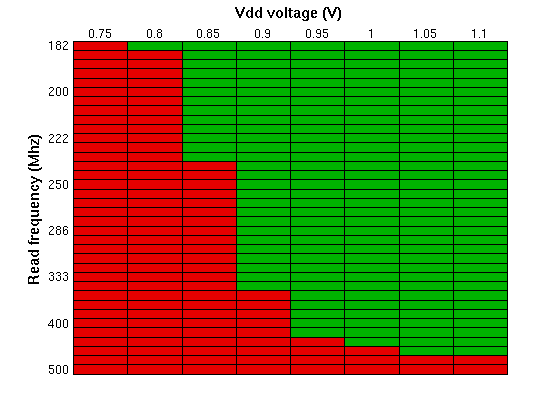
\includegraphics[scale=0.8]{../fig/hfdst-final-vddspeed.png}
  \caption{Resultaten speed-vdd test}
  \label{fig:speedvdd}
\end{figure}

Verder kan men ook zien dat de schakeling een voedingspanning hoger of gelijk aan 0.8V nodig heeft om correct te kunnen werken. De verklaring hiervoor kan gezien worden in figuur \ref{fig:vblvdd}. Deze figuur stelt de distributie voor van de bitlijn spanningen van een cell in RHS, de referentie cellen en een cell in LRS in functie van verschillende voedings spanningen. Er kan duidelijk gezien worden dat bij het verlagen van de voedings spanningen deze distributies dichter bij elkaar komen te liggen en dat een voedingspanning van 0.8V wel degelijk een limiet is. Aangezien de extremas van de distributies bij een voedingspanning van 0.8V zo dicht bij elkaar zitten, word er verder verwacht dat bij deze spanning de schakeling ook ocasioneel zal falen door dat de senseamplifier ontworpen is voor een $\Delta V$ van 35mV. Dit is echter niet opgedoken in de 100 montecarlo simulaties.
Als men naar de bitlijn voltage distributies kijkt voor een voedingspanning van 1V zal men opmerken dat deze niet de zelfde zijn als dezelfde distributie die getoont werden in het hoofdstuk van de last impedatie (figuur \ref{fig:distswitch}). Dit komt door dat men in de speed-vdd test niet wacht to de bitlijn volledig is opgeladen, wat een tijds winst oplevert. Ook werd er in het hoofdstuk van de last impedatie voor gestelt dat er een energie winst zou bereikt kunnen worden door een andere last te kiezen (sectie \ref{anderelast}). Hoewel dit mogelijk is, heeft dit wel als nadeel dat de schakeling minder tolerant zal zijn voor voedingspanning verschillen. Ten slotte moet ook vermeld worden dat de speed-vdd test uitgevoerd werd op een (spice) temperatuur van $30^{\circ}\mathrm{C}$. Moest deze schakeling worden geimplementeert in een processor is de kans groot dat dit onderhevig zal zijn aan temperaturen tussen de $30^{\circ}\mathrm{C}$ en $60^{\circ}\mathrm{C}$ wat ook een tragere leest snelheiden zal opleveren. Hoe traag, werd echter niet onderzocht.

\begin{figure}[!ht]
  \centering
  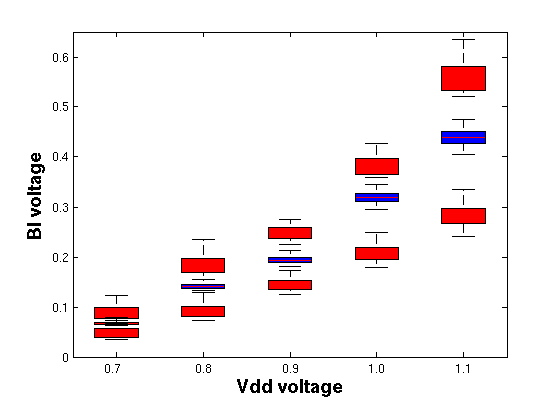
\includegraphics[scale=0.8]{../fig/hfdst-final-vddbl.png}
  \caption{Bl spanningen ifv Vdd}
  \label{fig:vblvdd}
\end{figure}

Het totale energie verbruik van een leescyclus bij een voeding spanning van 1V is gemiddelt 0.51pJ. Hier bij gaat 25\% van de energie naar de logic, 2\% naar de senseamplifier, 65\% naar de bitlijnen en 8\% naar de buffers. Hier bij werden de buffers in de decoders bij de logic gerekent.

\section{Besluit}
